% 
% Annual Cognitive Science Conference
% Sample LaTeX Paper -- Proceedings Format
% 

% Original : Ashwin Ram (ashwin@cc.gatech.edu)       04/01/1994
% Modified : Johanna Moore (jmoore@cs.pitt.edu)      03/17/1995
% Modified : David Noelle (noelle@ucsd.edu)          03/15/1996
% Modified : Pat Langley (langley@cs.stanford.edu)   01/26/1997
% Latex2e corrections by Ramin Charles Nakisa        01/28/1997 
% Modified : Tina Eliassi-Rad (eliassi@cs.wisc.edu)  01/31/1998
% Modified : Trisha Yannuzzi (trisha@ircs.upenn.edu) 12/28/1999 (in process)
% Modified : Mary Ellen Foster (M.E.Foster@ed.ac.uk) 12/11/2000
% Modified : Ken Forbus                              01/23/2004
% Modified : Eli M. Silk (esilk@pitt.edu)            05/24/2005
% Modified : Niels Taatgen (taatgen@cmu.edu)         10/24/2006
% Modified : David Noelle (dnoelle@ucmerced.edu)     11/19/2014
% Modified : Roger Levy (rplevy@mit.edu)     12/31/2018



%% Change "letterpaper" in the following line to "a4paper" if you must.

\documentclass[10pt,letterpaper]{article}

\usepackage{cogsci}

\cogscifinalcopy % Uncomment this line for the final submission 

% \usepackage{times}
% \cogscifinalcopy % Uncomment this line for the final submission 


% \usepackage{pslatex}
\usepackage{times}
\usepackage{apacite}
\usepackage{float} % Roger Levy added this and changed figure/table
                   % placement to [H] for conformity to Word template,
                   % though floating tables and figures to top is
                   % still generally recommended!

%\usepackage[none]{hyphenat} % Sometimes it can be useful to turn off
%hyphenation for purposes such as spell checking of the resulting
%PDF.  Uncomment this block to turn off hyphenation.
\usepackage{graphicx}
% \usepackage{fontspec}
\usepackage{amsmath}
\usepackage{amssymb}
\usepackage{booktabs}
\usepackage{xcolor}
\usepackage{lipsum}
\usepackage{multicol}
\usepackage{multirow}
\usepackage{epigraph}
\usepackage{natbib}
\usepackage{misra}
\usepackage{mathbbol}
\usepackage[OT1]{fontenc}
% \usepackage{natbib}

% \DeclareSymbolFont{letters}     {OML}{cmm} {m}{it}
% \DeclareMathAlphabet\mathcal{OMS}{cmsy}{m}{n}
% \SetMathAlphabet\mathcal{bold}{OMS}{cmsy}{b}{n}
% \renewcommand\sfdefault{cmss}

\definecolor{yello}{HTML}{ffb677}
\definecolor{blu}{HTML}{005082}
\definecolor{purpl}{HTML}{726a95}
\definecolor{orang}{HTML}{ff9a76}
\definecolor{tealish}{HTML}{1aa6b7}

\newcommand\BibTeX{B\textsc{ib}\TeX}

\newcommand{\ake}[1]{\textcolor{blue}{$_{AE}$[#1]}}
\newcommand{\km}[1]{\textcolor{purple}{$_{KM}$[#1]}}
\newcommand{\todo}[1]{\textcolor{purple}{$_{todo}$[#1]}}
\newcommand{\new}[1]{\textcolor{blu}{#1}}
\newcommand{\blank}{$\rule{0.6cm}{0.15mm}$}

\newcommand{\source}{\mathcal{S}}
\newcommand{\adaptation}{\mathcal{A}}
\newcommand{\generalization}{\mathcal{G}}
\newcommand{\concepts}{\mathcal{C}}
\newcommand{\properties}{\mathcal{P}}
\newcommand{\true}{\mathsf{True}}
\newcommand{\false}{\mathsf{False}}

\newcounter{argument}
% \counterwithin{argument}{equation}
\Roman{argument}
\newenvironment{argument}[2]{\refstepcounter{argument}\equation\begin{tabular}{@{}l@{}}
        #1 \\ \midrule #2
    \end{tabular}}{\tag{\roman{argument}}\endequation}


% \newcommand{\induction}[2]{% \logicarg{<premise>}{<conclusion>}
% \begin{equation}
%     \begin{tabular}{@{}l@{}}
%         #1 \\ \midrule #2
%     \end{tabular}%
% \end{equation}
% %   \begin{tabular}{@{}l@{}}
% %     #1 \\ \midrule #2
% %   \end{tabular}%
% }


\setlength\titlebox{4.5cm}
% You can expand the titlebox if you need extra space
% to show all the authors. Please do not make the titlebox
% smaller than 4.5cm (the original size).
%%If you do, we reserve the right to require you to change it back in
%%the camera-ready version, which could interfere with the timely
%%appearance of your paper in the Proceedings.

% \raggedbottom
\setlength{\parskip}{0pt}
\makeatletter
\renewcommand{\paragraph}{%
  \@startsection{paragraph}{4}%
  {\z@}{1ex \@plus 1ex \@minus .2ex}{-1em}%
  {\normalfont\normalsize\bfseries}%
}
\makeatother

\title{A Property Induction Framework for Neural Language Models}
 
\author{
{\large \bf Kanishka Misra,$^\textbf{1}$ Julia Taylor Rayz,$^\textbf{1}$ and Allyson Ettinger$^\textbf{2}$}\\
\texttt{kmisra@purdue.edu, jtaylor1@purdue.edu, aettinger@uchicago.edu} \\
  $^1$Department of Computer and Information Technology,
  Purdue University, IN, USA \\
  $^2$Department of Linguistics, University of Chicago, IL, USA
}

\begin{document}

\maketitle


\begin{abstract}
To what extent can experience from language contribute to our conceptual knowledge? 
Computational explorations of this question have shed light on the ability of powerful neural language models (LMs)---informed solely through text input---to encode and elicit information about concepts and properties. To extend this line of research, we present a framework that uses neural-network language models (LMs) to perform property induction---a task in which humans generalize novel property knowledge (\textit{has sesamoid bones}) from one or more concepts (\textit{robins}) to others (\textit{birds}). Patterns of property induction observed in humans have shed considerable light on the nature and organization of human conceptual knowledge. Inspired by this insight, we use our framework to explore the property inductions of LMs, and find that they show an inductive preference to generalize novel properties on the basis of category membership, suggesting the presence of a taxonomic bias in their representations.
% Our findings suggest that LMs indeed show strong sensitivity in generalizing novel properties to 
% on how LMs use the conceptual knowledge they encode to generalize beyond their training experience. To this end, we present a framework that adapts LMs to perform property induction---the task of projecting novel property information (\textit{can dax}) from one or more concepts (\textit{robin}) to a broader set of concepts and categories (\textit{crows, sparrows}). Using this framework, we investigate the extent to which LMs show an inductive preference to generalize novel properties on the basis of category membership.
% Investigations into \textit{property induction}---a task in which humans generalize novel property knowledge (\textit{has sesamoid bones}) from one or more concepts (\textit{robins}) to others (\textit{birds})---have shed light on the nature of human conceptual knowledge, and how it is organized. Inspired by this insight, we present a framework that uses neural-network language models (LMs) to perform property induction.
% To what extent can experience from language contribute to our intuitive understanding \ake{rephrase ``intuitive understanding'' to something more specifically related to the questions?} of the world? Computational explorations of this question have shed light on the ability of powerful neural language models (LMs)---informed solely through text input---to encode and elicit information about concepts and properties. We extend this line of research by asking how LMs use the conceptual knowledge they encode to generalize beyond their training experience. To this end, we present a framework that adapts LMs to perform property induction---the task of projecting novel property information (\textit{can dax}) from one or more concepts (\textit{robin}) to a broader set of concepts and categories (\textit{crows, sparrows}). Using this framework, we investigate the extent to which LMs show an inductive preference to generalize novel properties on the basis of category membership.

\textbf{Keywords:} 
property induction; language models; semantic cognition; generalization; conceptual knowledge
\end{abstract}


\section{Introduction}
% There has recently been a growing interest in exploring the potential of language as a contributor to knowledge about mental representations of objects and events (concepts), the class of entities they pick out (categories), their attributes (properties) and inter-relations -- collectively referred to as conceptual knowledge \citep{murphy2004big, machery2009doing}.
There has recently been a growing interest in exploring the limits and potential of language as an environment for learning conceptual knowledge \citep{elman2004alternative, lupyan2019words}---knowledge that encompasses mental representations of everyday objects/events, and their properties and interrelations, that together inform our intuitive understanding of the world \citep{murphy2004big, machery2009doing}.
% Under this view, words are interpreted to act as \textit{cues} to meaning, where instead of directly and explicitly mapping onto concepts, they activate and eventually help build one's conceptual repertoire \citep{elman2004alternative, lupyan2019words}.
% On the basis of this claim, several inquiries have aimed to understand the extent to which computational models that acquire semantic representations through text alone can capture conceptual knowledge \citep{derby-etal-2019-feature2vec, weir2020probing}.
Computational explorations of this claim often study the extent to which models that learn semantic representations through text alone can capture conceptual knowledge \citep{lucy-gauthier-2017-distributional, forbes2019neural, bhatia2020transformer}.
% \ake{consider making this a new paragraph} 

A hallmark feature of the conceptual knowledge acquired by humans is its capacity to facilitate inductive generalizations: inferences that go beyond available data to project novel information about concepts and properties \citep{osherson1990category, chater2011inductive, hayes2018inductive}.
For example, our knowledge of taxonomic specificity is reflected when we generalize a novel property of a concept (e.g., \textit{robins have T9 hormones}) more strongly to taxonomically close concepts (\textit{sparrows have T9 hormones}) than to more taxonomically distant concepts (\textit{tigers have T9 hormones}).
Inductive generalizations about novel properties (also called \textit{property induction}) therefore provides a context within which we can explore the nature of 
% models' 
agents' understanding of conceptual knowledge.
% Specifically, this context can be used to shed light on the inductive preferences of models --
% e.g., when told ``\textit{dolphins have blickets,}'' a model that activates category-membership knowledge will likely project the new property to mammals as opposed to fish, but the reverse will be observed if it activates behavioral or visual knowledge.
To this end, we develop an analysis framework that uses neural network-based language models (LMs, henceforth) to perform property induction and use this framework to study concept representation in these models.
Our framework consists of two stages. 
In the first stage, we train LMs to evaluate the truth of sentences expressing property knowledge (e.g., \textit{a cat has fur} $\rightarrow$ True, \textit{a table has fur} $\rightarrow$ False). 
In the second stage, we use these property-judgment models to test how the representations from the underlying LMs drive inductive generalization of novel properties -- e.g., \textit{can fep, can dax,} etc.


% Each stage of our framework sheds light on different aspects of LMs' conceptual knowledge and its contribution to the generalizations made by them.
Each stage of our framework sheds light on different aspects of the conceptual knowledge captured by LMs.
Using the first stage, we test the extent to which LMs support judgement of whether a property applies to a concept, even when that property has not been seen in task-specific fine-tuning. 
We find that LMs perform substantially above chance, consistent with the conclusion that they are able to rely on generalizable property knowledge to assess truth of concept-property associations.
In the second stage, we use this property judgment framework to study how knowledge representation in the base LMs drives inductive generalization with respect to entirely novel properties. We focus specifically on whether models' inductive preferences indicate reliance on taxonomic information, by testing whether models prefer to generalize within rather than outside of taxonomic categories. To do this, we teach our property-judgment models novel property information such as \textit{robins can dax} and then test the extent to which they prefer generalizing this novel property to other birds
% (e.g. \textit{sparrows can dax}) 
more strongly than to non-birds.
% .(e.g., \textit{tigers can dax}) 
% \ake{now that I added these examples earlier we might be able to remove them here}.
We find that models indeed show a preference to generalize new property knowledge on the basis of taxonomic category membership, suggesting that the models have acquired and represented some version of taxonomic features on which they rely to project novel information.
This taxonomic preference also persists when we account for the extent to which category-based generalization is reflected in the property-judgment training data, suggesting that these inductive generalizations reflect more than simple fine-tuning statistics.

Our LM-based account of property induction contributes to the field in three primary ways. 
On the basis of the goals of the task, our framework focuses on reasoning where conclusions do not deductively follow from the premise, unlike the goals of the more commonly-used task of natural language inference \citep{bowman2015large}, and it therefore allows for testing of human-like inferences that are yet to be studied in LMs.
% First, our modeling framework allows for testing of human-like inferences that are fundamentally different from the more commonly-used task of natural language inference \citep{bowman2015large}, which is exclusively deductive in nature. 
Next, as we show below, our framework opens a new window into exploring how large neural networks models of language generalize beyond their training experience, complementing inquiries of models' inductive bias with respect to syntactic structure \citep{mccoy2020does} and ``universal linguistic constraints'' \citep{mccoy2020universal}. Finally, this work advances research aiming to diagnose the nature and extent of conceptual knowledge in LMs \citep{da-kasai-2019-cracking,forbes2019neural,weir2020probing, bhatia2020transformer} by additionally focusing on how knowledge present in LM representations drives the generalizations they make.

\section{Testing Property Induction with Arguments}
% \km{Property induction is often studied with the help of arguments -- set of statements structured as premise and conclusion. General vs specific based on taxonomic status of the premise and conclusion concepts.}
Property induction is often studied experimentally in humans through the use of arguments, represented in the following premise-conclusion format, as popularized by \citet{osherson1990category}:
\begin{argument}
{A robin can dax.}{All birds can dax.}\label[arg]{arg:example}
\end{argument}
\Cref{arg:example} is read as \textit{``A robin can dax. Therefore, all birds can dax.''}
The subject of the premise sentence (\textit{robin}) is referred to as the premise concept (similarly, if there are multiple premises, we have a set of premise concepts), while that of the conclusion is called the conclusion concept.
Representing induction stimuli as arguments allows one to use the notion of ``argument strength,'' which quantifies the degree to which a human subject's belief in the premise statements strengthens their belief in the conclusion \citep{osherson1990category}.
%  \ake{sentence tying this to what you will do with models?}\km{difficult to add without explaining in detail, but I will try my best to summarize as briefly as I can} \ake{just super simple like ``These patterns of generalization reflect organization of human conceptual knowledge, and we use this framework to test conceptual knowledge in LMs'' }\km{I feel if we want to say that it should go in the intro, which we kind of say already? with the above paragraph I primarily wanted to discuss the format of stimuli} \ake{if you have space for it that kind of repetition is good to help people keep track of how everything connects}
% \km{ah okay! makes sense} 

In many cases, researchers control the type of novel properties provided to participants by using \textit{blank} properties -- properties that are synthetically created and are therefore unknown to participants, maximizing the chances that they will use their knowledge of the relations between the premise and conclusion concepts to make generalizations \citep{rips1975inductive, osherson1990category, murphy2004big}. In our property induction experiments, we simulate blank properties by using nonce words to synthetically construct novel properties---e.g., \textit{can dax}, \textit{is vorpal}, etc and use them to explore knowledge of conceptual relations in LMs.
% \subsection{Connectionism and Property Induction}
% \km{LMs are contemporary implementation of the parallel distributed processing approach, trained to learn from text sequences. 
% Discuss the NN model of \citep{rogers2004semantic} and their operationalization of induction. Premise of connectionism is that structure needed to learn and represent knowledge is learned from the statistics of the environment, and induction is one of the many important phenomena that is tested and simulated. by providing an account of induction in LMs, one can shed light on how well knowledge picked up by LMs from the statistics of text data is put to use.
% We can use the framework to narrow in on specific hypotheses that can be tested by forming an inductive argument and testing whether the LM generalizes according to the hypothesis.}

\section{The Framework}

% \ake{one-sentence summary of what the framework is and what its purpose is: ``In order to test X, we develop a framework that Y. In this section we describe this framework.''}%\km{\citet{misra2021typicality} and other forms of candidate setups (NLI).}

% \ake{this paragraph feels out of place---the section should focus on the nature of the framework and what your motivation was, rather than going into a long explanation of another paper that's doing a different thing. How about you instead just say something like ``We choose this approach over simple cloze tasks in order to avoid X, observed in similar work by Misra et al.''} 
% \km{That makes a lot of sense! I will re-write this to do exactly that}
Computationally, property induction can be viewed as making conditional probability estimates about the conclusion ($c$), given some premise ($\pi$): $p(c\mid\pi)$.
We interpret this measure in our framework as a probability that a novel property is applied to a conclusion concept, by a model whose representations reflect the premise information.
This interpretation leads to two desiderata that our framework aims to satisfy: (1) the ability to make judgments about the association of concepts to properties, and (2) the ability to accept new property knowledge and then be queried to assess generalization or `projection' of this new property knowledge to additional concepts.
To satisfy (1), we fine-tune existing pre-trained LMs to classify as true or false sentences that associate concepts to properties---i.e., make property judgments. This automatically allows the models to estimate the probability that a property applies to a concept---as $p(\textit{``concept has property''} = \true)$. 
We use this approach rather than estimating simple sequence probabilities---which are relatively more straightforward to compute using LMs---in order to avoid surface-level confounds as observed in similar work by \citet{misra2021typicality}.
Next, to satisfy (2), we operationalize induction as the behavior of these LMs (now fine-tuned to make property-judgments) after adapting to new properties using standard backpropagation \citep{rumelhart1986learning}.
The motivation to use backpropagation to perform property induction is simple---it allows the integration of new information in the model by directly updating its representations, which encode knowledge used to inform how the model generalizes. 
Furthermore, the updates that backpropagation introduces in the model can be directly quantified, allowing us to explore numerically how models integrate new information in their representations.
% Due to itsackpropagation further allows use to  measurable by using metrics such as loss or accuracy, which allows us to shed light on how well the model integrates certain kinds of knowledge.
A similar operationalization of induction was used by the pioneering work of \citet{rogers2004semantic}, who reported inductive inferences made by their PDP model of semantic cognition by updating its weights to reflect novel information, which was provided after several steps of training on general conceptual knowledge derived from a toy-dataset of concepts and properties.
Similarly, \citet{van2018neural} adapt language models on novel syntactic structures to shed light on their syntactic adaptation capacities.

% \noindent
We now explain the two stages of our property induction framework in greater detail:

% To first encode the capacity to estimate probability measures for concept-property associations, we 

% \begin{align}
%     p(\textit{conclusion} \mid \textit{premise}, \Theta)\label{eq:conditional}
% \end{align}
% A related account of LM-based property induction, put forth by \citet{misra2021typicality} uses sequence probabilities elicited by LMs to estimate this measure, where the conclusion sentence is preceded by the premise sentence(s). Using this method, the authors shed light on whether LMs are sensitive to the \textit{typicality} of concepts \citep{rosch1975cognitive} by comparing the generative probability of a conclusion (e.g. \textit{all birds can dax}) when conditioned on a typical (e.g. \textit{a robin can dax}) versus an atypical premise (e.g., \textit{a penguin can dax}).
% % comparing typical (\textit{a robin can dax}) versus atypical premises (\textit{a penguin can dax}) for the same conclusion (\textit{all birds can dax}).
% While this method tests LMs in their natural environment of predicting sequences, it introduces the possibility of superficial confounds that influence the model's predictions. For instance, \citet{misra2021typicality} found LMs to produce high scores for the conclusion in two notable cases: (1) when the words of the premise were shuffled, suggesting their inability to compositionally reason about the premise; and (2) when the premise contained a random concept, suggesting that they were likely assigning high probability to the property phrase, simply because it was listed in the preceding context (i.e., being conducive to repeating input text).
% % \km{(while this method tests LMs in their natural environment of predicting sequences, it is susceptible to confounds.) }
% It is therefore unclear whether the model's representations are necessarily using conceptual knowledge to estimate word probability.
% One conclusion that can be drawn here is that this setup sheds more light on whether specific phenomena affect word prediction rather than whether the LM is necessarily performing induction, thereby necessitating alternate methods to simulate property induction.

% Informed by the potential issues in using sequence probabilities \citep{misra2021typicality}, 
% % as well as the insights from the connectionist account of  semantic cognition \citep{rogers2004semantic}, 
% we now present a dual-stage framework to perform property induction using LMs.

\subsection{Stage 1: Eliciting Property Judgments using LMs}
In the first stage, we constrain LMs to explicitly rely on property knowledge by distinguishing correct (\textit{cat has whiskers}) and incorrect associations (\textit{sparrow has whiskers}) between concepts and properties. 
We do this by fine-tuning LMs to classify sentences that express concept-property associations to be true or false. Importantly, as we will show in our first experiment, we fine-tune models in a way that keeps the evaluation sets disjoint in terms of properties---i.e., the model is trained to assess the properties \textit{has feathers, has a tail} and then tested on a distinct set of properties: \textit{can fly, has a beak}.
Therefore, in order to succeed on this task (i.e., minimize loss on a disjoint evaluation set), a model must rely on property knowledge encoded in its representations.
% -- i.e., it must have an inductive bias that favors knowledge about properties. 
Below we verify the extent to which the models are indeed able to draw on generalized property knowledge in order to succeed in this task. 
% This stage importantly relies on the existence of a repository of concepts ($\concepts$) and their properties ($\properties$).
% % that can be used to create sentences on the basis of which we tune the model's parameters.
% While we discuss the characteristics of one specific repository in the next section, assuming that $\concepts$ and $\properties$ do exist, 
Importantly, this stage assumes the presence of a repository of concepts ($\concepts$) and associated properties ($\properties$). 
We create sentences that express property knowledge by pairing concepts from $\concepts$ to properties from $\properties$. We then fine-tune the LM to classify these sentences as true or false. At the end of this stage, we have a trained model $\phi$ that takes as input a sentence $s$ and produces a probability score corresponding to the truth of s, $p_{\phi}(s = \mathsf{True})$, as internalized by the model.
\Cref{fig:framework}A describes the property judgment stage.
% \km{Instead of using sequence probabilities, we estimate \cref{eq:conditional} using a property judgment task.
% Specifically, we propose to tune the parameters of a given LM to explicitly classify whether a concept is correctly attributed its properties, i.e., predict the truth of sentences that link concepts and properties (\textit{a cat has fur}) in a binary-classification setup.}
% \km{ Doing so can impart a favorable inductive bias to the LM, in that its representations are relatively more constrained to rely on property knowledge to formulate the output as compared to when they were being used to perform word-prediction. Therefore, a successful property judgment model will have to rely on property knowledge in order to succeed at this task (which we test in our first experiment).
% }
% Doing so can impart a favorable inductive bias to the LM, in that its representations are relatively more constrained to rely on property knowledge to formulate the output as compared to when they were being used to perform word-prediction.
% \km{(Existence of a repository of conceptual knowledge..)
% We propose to estimate \cref{eq:conditional} using an explicit property judgment task.
% Specifically, we propose to fine-tune LMs to classify whether a concept is correctly linked to its properties in a sentence-based binary classification.
% }
% \km{
% Instead of estimating 
% Since both the premise and the conclusion are represented as natural language sentences, we can estimate the above measure by training LMs to make judgements about whether a concept can possess a given property.
% Specifically in this stage, we fine-tune LMs to classify sentences linking concepts to properties as true or false, i.e., in a binary classification setting.
% Doing so imparts a favorable inductive bias to the LM, in that their representations are more constrained to use property knowledge relative to when they were when used to perform word-prediction.}
\begin{figure*}[t!]
    \centering
    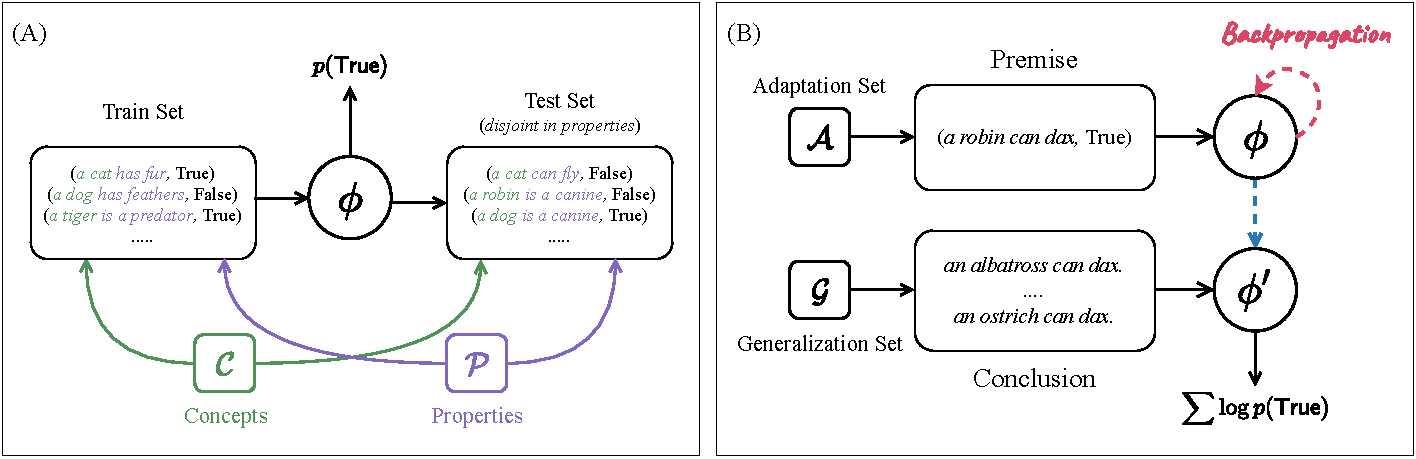
\includegraphics[width=0.8\textwidth]{inductionframeworkcogsci.pdf}
    \caption{\textbf{(A)} Property Judgment Stage describing the training of the property judgment model $\phi$ to make judgments of truth on sentences expressing concept-property assertions. Sentences created using the concept ($\concepts$) and property ($\properties$) data collected by \citet{devereux2014centre}; \textbf{(B)} Depiction of the Induction Stage, in this case, for testing the generalization from robin to all birds. Here, $\adaptation = \{\textsc{robin}\}$, $\generalization = \{\textsc{albatross}, ..., \textsc{ostrich}\}$, and the novel property being generalized is ``\textit{can dax}.''}
    \label{fig:framework}
\end{figure*}
\subsection{Stage 2: Induction as Domain Adaptation}
% We operationalize induction as 
In this stage, we use the fine-tuned model from the previous stage to perform property induction, which we operationalize as the behavior of the model after adaptation to new property knowledge via backpropagation \citep{rumelhart1986learning}.
% The motivation to use backpropagation to perform property induction is simple -- it allows the integration of new information in the model by directly interacting and updating its representations which seemingly encode knowledge that is used to inform how the model generalizes. 
% Furthermore, the updates that it introduces in the model can be quantified, allowing us to explore numerically how models integrate new information in their representations.
% % Due to itsackpropagation further allows use to  measurable by using metrics such as loss or accuracy, which allows us to shed light on how well the model integrates certain kinds of knowledge.
% A similar operationalization of induction was used by the pioneering work of \citet{rogers2004semantic}, who reported inductive inferences made by their PDP model of semantic cognition by updating its weights to reflect novel information which was provided after several steps of training on general conceptual knowledge derived from a toy-dataset of concepts and properties.
% Similarly, \citet{van2018neural} adapt language models on novel syntactic structures to shed light on their syntactic adaptation capacities.

An instance of property induction involves (1) a set of premise concepts (which we denote as the adaptation set $\adaptation \subset \concepts$); (2) a set of conclusion concepts (denoted as the generalization set $\generalization \subset \concepts$); and (3) a novel property being generalized from the premise to the conclusion.
% The content of these artifacts depends on the specific inductive phenomena being simulated.
We construct sentences that associate the novel property to the concepts in $\adaptation$ and $\generalization$, yielding the premise and conclusion stimuli, respectively (see Figure 1B).
To perform a round of property-induction, we first adapt the model $\phi$ to the premise sentences by using standard backpropagation, yielding an updated state of the model $\phi^{\prime}$, that correctly attributes the concepts in $\adaptation$ with the novel property.
We then freeze the parameters of $\phi^{\prime}$ and query it with the conclusion sentences to get the model's (log) probability of generalizing (or ``projecting'') the novel property to the concepts in $\generalization$.
An example of this stage is shown in \Cref{fig:framework}B.
% To formalize this notion, we denote the source concepts by $S$
% While every induction experiment is idiosyncratic to the phenomena of interest, we will use \cref{arg:example} as the running example.
% \km{backpropagation as mechanism to integrate new knowledge into the representations of model obtained in the previous stage.}
% \subsection{Using the Framework}
% To measure the strength of projecting the novel property to a given set of generalization concepts, we use log-probabilities from the updated model $\phi^{\prime}$
% An instance of property induction can involve the testing of generalization to one or more concepts.
We denote the model's log-probability on the generalization set as the ``generalization score'' ($\mathbb{G}$)---the strength of projecting the novel property to a set of one or more concepts in the generalization set:
% We compute the argument strength for instances with single concept in the generalization set as:
% \begin{align*}
%     AS = \log p_{\phi^{\prime}}(\textit{``c}\textit{ has property X''} = \true)
% \end{align*}
% For cases when the generalization set consists of multiple concepts (e.g., superordinate categories such as \textsc{bird}),
% It is computed as the average log-probability of generalizing the novel property to all concepts in the generalization set:
\begin{align}
    \mathbb{G} = \frac{1}{n}\sum_{\textit{c}_i \in \mathcal{G}} \log p_{\phi^{\prime}}(\textit{``c}_i\textit{ has property X''} = \true)\label{eq:genscore}
\end{align}

We now use components of this framework in two experiments---one for each stage in the framework.

\section{Property Judgment Experiment}
This experiment focuses on the first stage of the proposed induction framework. Here, we fine-tune pre-trained LMs to judge the truth of sentences that link concepts to properties. 
Since our setup keeps the training and the evaluation data perfectly disjoint in terms of properties (as we will show), we expect that a model must constrain its parameters to rely on previously encoded property knowledge in order to succeed. Here we test the extent to which this indeed is the case. 
\paragraph{Property Knowledge Data}
To construct sentences that express property knowledge, we rely on a property-norm dataset collected by the Cambridge Centre for Speech, Language, and the Brain \citep[CSLB;][]{devereux2014centre}.
The CSLB dataset was collected by asking 123 human participants to annotate properties for a set of 638 concepts, and this dataset has been used in several
% a number of 
studies focused on investigating conceptual knowledge in word representations learned by computational models of text \citep[e.g., ][]{lucy-gauthier-2017-distributional, da-kasai-2019-cracking, bhatia2020transformer}.
Property-norm datasets consist of data about what properties apply to a given concept, and therefore lack negative concept-property associations. 
As a result, the aforementioned works \citep{lucy-gauthier-2017-distributional, da-kasai-2019-cracking, bhatia2020transformer} randomly sample concepts for which a particular property was not elicited and take them as negative instances for that property (e.g., using \textsc{table, chair, shirt} are negative instances for the property \textit{can breathe}). These negative instances can then be used in a standard machine-learning setting to evaluate a given representation-learning model.

% \ake{The description of all of this data cleaning maybe belongs in its own section, if it's not a part of this experiment per se?} 
Upon careful inspection of the CSLB dataset, we found that the above practice may unintentionally introduce incorrect data.
Datasets such as CSLB are collected through human elicitation of properties for a given concept,
so it is possible for inconsistencies to arise. One way this may happen is when some participants choose not to include properties that are obvious for the presented concept (e.g., \textit{breathing} in case of living organisms), while other participants do, resulting in an imbalance that can be left unaccounted for.
% so it is possible that there are cases when a property was not elicited for some concepts -- we suspect 
We found that this was indeed the case: e.g., the property \textit{has a mouth} was only elicited for 6 animal concepts (out of 152), and so all other animals in the dataset would have been added to the negative search space for that property during sampling, thereby propagating incorrect and incomplete data. This indicates a potential pitfall of directly using property-norm datasets to investigate semantic representations---and suggests that prior evaluations and analyses \citep{lucy-gauthier-2017-distributional, da-kasai-2019-cracking, bhatia2020transformer} may have falsely rewarded or penalized models in some cases.
To mitigate this issue, we first selected the concept categories \citep[hand-annotated by][e.g., \textsc{bird, vehicle, tree}, etc.]{devereux2014centre} that had at least 9 concepts in the dataset and were not labelled as ``miscellaneous,'' resulting in 24 different categories with a total of 538 unique noun concepts, and 4{,}970 unique properties.
Next, we manually removed concepts and properties that contained proper nouns (e.g., \textsc{rolls-royce}, \textit{is in Harry Potter}), stereotypical or subjective data (e.g., \textit{is meant for girls}, \textit{is ugly}), and explicit mentions of similarity or relatedness (e.g., \textit{is similar to horse}). We further normalized properties that were paraphrases of each other (e.g., \textit{is used to flavor, does flavor} $\rightarrow$ \textit{is used to flavor}). This resulted in 530 concepts and  3{,}873 properties.
Again through manual annotation, we further identified a total of 234 properties that were incompletely annotated (i.e., those that were associated with certain concepts but were omitted for many relevant concepts during data collection -- e.g., \textit{can grow} was missing for all invertebrates) and we extended the coverage for these properties. 
While this may seem like a small number (6\% of the valid properties), it greatly increases the total number of concept-property pairs (from 13{,}355 pairs to 22{,}046: an increase of 65\%) since many of the incompletely labelled properties were applicable across several categories (e.g., \textit{has a mouth, can grow,} etc).

% Using the 530 concepts ($\concepts$) and 3{,}873 properties ($\properties$), we generate 
Instead of randomly sampling negative concepts for each of our 3{,}873 properties ($\properties$), we sample concepts that are similar to those associated with a particular property---e.g., for the concept \textsc{zebra}, we want to use \textsc{horse} for a negative sample rather than something random such as \textsc{table}.
By doing so, we make the property judgment tasks increasingly difficult, increasing the chances that the models that we obtain from this stage are indeed focusing on conceptual knowledge to make property judgments instead of relying on simpler superficial cues such as lexical co-occurrence \citep{mccoy-etal-2019-right}.  
To this end, we first create a taxonomy of our 530 concepts ($\concepts$) by identifying their WordNet \citep{miller1995wordnet} senses.
Then, for each property---associated with $k$ different concepts---we perform a weighted sampling from the set of leftover concepts (with size $530-k$), where each leftover concept is assigned a weight proportional to its \textit{Wu-Palmer similarity} \citep[a commonly used taxonomic similarity computed over the subset of wordnet taxonomy;][]{wu-palmer-1994-verb} with every concept associated with the property. 
This results in a set of negative concept-property pairs that is equal in size to our positive set.
We then follow the method outlined by \citet{bhatia2020transformer} to convert our concept-property pairs into 22{,}046 true and 22{,}046 false property knowledge sentences.
% \footnote{this involves minimal modification since most of our properties are already represented as well-formed verb-phrases.}
Finally, we split our 44{,}092 sentence-label pairs into training, validation, and testing sets (80/10/10 split), such that the testing and validation sets are only composed of properties that have never been encountered during training (properties between training and validation sets are also disjoint). 
We do this to avoid data leaks, and to ensure that we evaluate models on their capacity to learn property judgment as opposed to memorization of the particular words and properties in the training set. 
% task.
We make our entire filtering pipeline and negative sample generation algorithm available at (url hidden).

\paragraph{Tested LMs}
While our framework can be applied to any neural language model, we present results from fine-tuning three pre-trained LM families, based on the precedent of using these models in standard sentence classification tasks \citep{wang2018glue}: BERT \citep{devlin-etal-2019-bert}, RoBERTa \citep{liu2019roberta}, and ALBERT \citep{lan2019albert}. 
% The models were selected on the basis of their \km{(preferred)} use in standard sentence classification tasks in the NLP community \citep{wang2018glue}. 
All three models use the transformer architecture \citep{vaswani2017attention}, and are trained to perform masked language modeling: the task of predicting words in context in a cloze-task setup, where models have access to words to the left and right of the masked word. 
We report results using the largest models in each of the three families---BERT-large, RoBERTa-large, and ALBERT-xxl---since these variants had the best performance in our preliminary experiments.
% \paragraph{Fine-tuning}
We fine-tune each of the three models on the property knowledge data by minimizing their binary cross-entropy loss on the training set using the Adam optimizer \citep{kingma2014adam}.
We tune the hyper-parameters (such as learning rate) on the basis of the validation set, and finally evaluate the three adapted models on the test set using the F1 score.
% Let $\mathcal{C}_{\properties_i}^{\prime}$ be the set of concepts that do not possess a particular property $\properties_i$
% Then, for each property, we first split $\concepts$
% \begin{align}
%     \frac{(n+1)\times \texttt{depth}(\texttt{lcs}(p_1, \dots, p_n, r_i))}{\texttt{depth}(p_1) + \dots + \texttt{depth}(p_n) + \texttt{depth}(r_i)}
% \end{align}
% In order to get models that are more conducive to rely on conceptual knowledge to make property judgments instead of superficial cues \citep{mccoy-etal-2019-right}, we 

% \km{CSLB norms \citep{devereux2014centre} consisting of n concepts and m properties. How this dataset has traditionally been used in probing experiments -- for each category, all members that do not have an associated production frequency are set to False. Upon careful inspection, we find that this practice can introduce unintended problems -- ``absence of evidence vs. evidence of absence''}

% \km{Train test split creation: negative instances created by sampling similar concepts that do not possess the properties, using a taxonomic similarity metric (details in supplementary material)}

\paragraph{Results}
\Cref{tab:f1} shows the performance of the three models in our property judgment experiments. 
% \km{generally high scores, suggesting that to an extent the model learn to rely on concept knowledge through this true-false setup.}
We find that all three models show similarly high performance on validation (0.79-0.82) and test sets ($\approx$ 0.79 throughout), suggesting strong capacities of all three models to assess the application of properties to concepts. Notably, the ALBERT-xxl model shows the same performance as BERT-large and RoBERTa-large despite having $\approx$130M fewer parameters, suggesting that this property knowledge can be encoded in smaller models with more efficient use of parameters.

\begin{table}[t!]
\vspace{-1em}
\def\arraystretch{1.15}
\centering
\caption{Performance (F1 scores) of the three adapted models on Validation and Test sets, each of which is disjoint in terms of properties from the Training set. Chance F1 = 0.50}
\label{tab:f1}
\vspace{0.5em}
\begin{tabular}{|l|c|c|c|}
\hline
\textbf{Model} & \textbf{Params} & \textbf{Val. F1} & \textbf{Test F1} \\ \hline
ALBERT-xxl     & 212M            & 0.81             & 0.79    \\
BERT-large     & 340M            & 0.79             & 0.79    \\
RoBERTa-large  & 345M            & 0.82    & 0.79    \\ \hline
\end{tabular}
\end{table}

\section{Investigating Taxonomic Generalizations in LMs using Property Induction}
% Using the three property-judgment models from the previous experiment, we now demonstrate how our induction framework can be used to answer questions related to the models' inductive behavior, and by extension the kinds of knowledge they may be putting to use in making generalizations beyond available data.
% As a case-study, we will focus on inductive generalizations made on the basis of taxonomic relations between concepts and ask whether the models use knowledge of category-membership to make project newly provided properties.
Taxonomic relations between concepts have an important role in studies of human inductive reasoning.
Early evidence from \citet{gelman1986categories} indicated a strong preference of children and adults, when making generalizations about new and unfamiliar properties, to do so based on the structure of biological taxonomies and category membership.
\begin{figure*}[h]
    \centering
    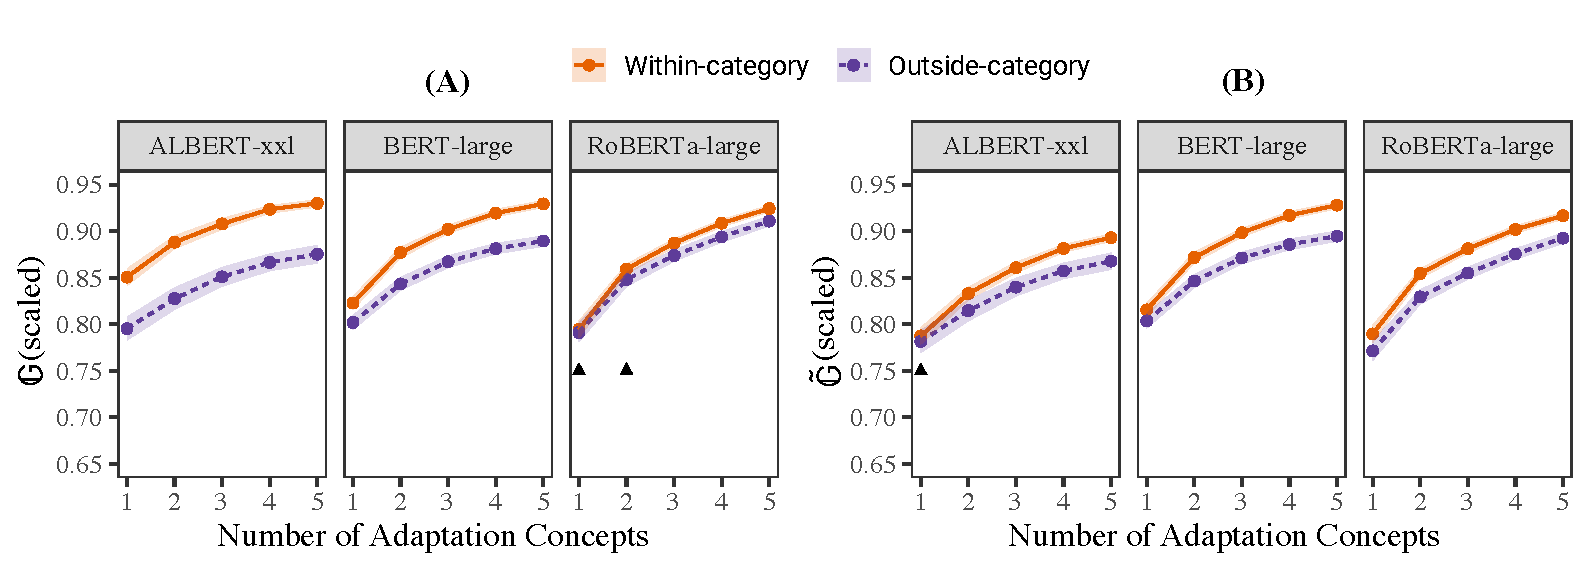
\includegraphics[width=\textwidth]{withwithoutoverlaps.pdf}
    \caption{\textbf{(A):} Results from Taxonomic Generalization experiment showing generalization scores ($\mathbb{G}$) between ``Within-category'' and ``Outside-category'' generalization sets across various number of adaptation concepts. \textbf{(B):} Same depiction as \textbf{(A)} but with the the effect of property-overlaps between adaptation and generalization concepts removed. Cases where the difference between $\mathbb{G}$-scores of within versus outside category sets are not significant under $\alpha = .05$ are marked with a `$\blacktriangle$'}
    \label{fig:taxonomicresults}
\end{figure*}
% \citet{gelman1986categories} were one of the first ones to observe the role of taxonomic relations emerge in patterns of induction in children and adults. 
% In their experiments, \citeauthor{gelman1986categories} first displayed a picture of a flamingo to their subjects and informed them that it had a ``right aortic arch,'' then displayed a picture of a bat and told them that it had a ``left aortic arch.'' 
% When later shown a picture of a blackbird (that visually resembled the bat more than it did the flamingo), the subjects attributed it ``a right aortic arch'', indicating a preference for biological taxonomies in their inductive judgments.
Building on this, \citet{osherson1990category} documented 13 separate taxonomic phenomena that influenced inductions made by humans.
Inspired by these pioneering works, we demonstrate how our property induction framework can be used to test whether a similar taxonomic bias is reflected in the LMs used to train the above property judgment models. 
For instance, if a model is provided with a new property---e.g., \textit{can fep}---that is associated with the concept \textsc{cat}, to what extent do its representational biases cause it to prefer generalizing or projecting this property to other mammals rather than to fish? 
% Furthermore, the notion of \textit{premise monotonicity} \citep{osherson1990category} suggests that the inductive strength of ``\textit{all mammals can fep}'' should increase with an increase in the number of premise concepts (i.e., the generalization score for \{\textsc{cat}, \textsc{cow}\} to mammals should be greater than that from \textsc{cat} to mammals). 
% This allows us to shed light on whether the representations of these models support generalizations based on category membership.


\paragraph{Data} We restrict our analysis to the animal-kingdom subset of the concepts in our modified property-norm data, corresponding to a total of 152 concepts.
We first select the top six categories within this subset: \textsc{mammal} (52), \textsc{bird} (36), \textsc{insect} (18), \textsc{fish} (14), \textsc{mollusk} (8), and \textsc{reptile} (7).
Each instance in this experiment starts with a focus category (of size $m$) from which we sample $n$ concepts to create the adaptation set, and use the remaining $m-n$ to create the ``Within-category'' generalization set.
Similarly, we create the ``Outside-category'' generalization set by sampling the top $m-n$ animal concepts that are outside the focus category, on the basis of their average cosine similarity with the concepts in the adaptation set (calculated using the representations from the embedding layer of the given model). We use this weighted sampling technique in lieu of simple random sampling in order to increase our confidence that observed differences can be attributed to category differences and not to general similarity properties.
% test differences between within and outside category generalization at their intuitive limits -- 
% it is reasonable to assume that representational similarity may play a role in the model's generalizations, so 
% having our outside-category set be similar to the adaptation set as opposed to being randomly sampled allows us to be more confident in our conclusions.
We repeat this sampling process 10 times, for $n = 1, \dots, 5$ adaptation concepts, and 8 novel properties: verb phrases created using nonce words (\textit{can dax, can fep, has blickets, has feps, is a tove, is a wug, is mimsy, is vorpal}). In total, we have 2{,}400 samples per model.
%$6 \times 10 \times 5 \times 8 = 2400$
\paragraph{Method}
In each trial, we pass the adaptation set to the models and let them minimize their loss (using the same optimizer state obtained at the end of the property judgment training phase) until they reach perfect accuracy. Then for each model, we compute $\mathbb{G}$ for both of our generalization sets as shown in \cref{eq:genscore}. 
\Cref{fig:taxonomicresults}A shows the average $\mathbb{G}$ (over all properties, re-scaled to lie between 0 and 1) across the number of adaptation concepts.

\paragraph{Results and Analysis}
We expect models with a preference for category-based generalization to have greater average $\mathbb{G}$ values for the ``Within-category'' set than for the ``Outside-category'' set.
From \Cref{fig:taxonomicresults}A, we see that ALBERT-xxl and BERT-large consistently 
show this pattern (differences between ``Within-category'' and ``Outside-category'' were significant at $p<.001$ using a t-test), suggesting that these models do show taxonomic biases in property generalization. This preference is substantially smaller for RoBERTa-large (with non-significant differences between generalization to within versus outside category for $n=1,2$), suggesting relative indifference in that model to taxonomic vs. representational similarity when it comes to extending new property knowledge to concepts outside the adaptation set.
We also observe that the average generalization score in both categories increases with an increase in the number of adaptation concepts. Notably, this is also robustly observed in humans (characterized as the \textit{premise monotonicity effect} by \citeauthor{osherson1990category})---however, we do not focus on this effect, as it is relatively expected that data-driven models will be more confident in their outputs as the number of samples provided to them increases.

Although the properties provided to the model are ones that they have never seen during training in the property-judgment stage, one may wonder to what extent the models' inductive behavior can be explained based on taxonomically similar concepts simply being more likely to share properties within the property-judgment training stage---this could call into question how much these generalization patterns tell us about the underlying concept knowledge in the LMs.  
% overlap in properties between the concepts of the adaptation set and each of the generalization sets? 
Under the connectionist perspective of property induction \citep{sloman1993feature, rogers2004semantic}, the strength of generalization (of a novel property) to a concept is proportional to the overlap in properties between the premise (adaptation set) and the conclusion (generalization set).
We can reasonably expect this to translate to the models that we use here,
% ---they essentially are sophisticated successors of connectionist models---
especially since they are trained to predict the presence and absence of properties.
It is therefore revealing to understand the extent to which models' preference toward category-based generalization persists if we remove the component of their generalizations that is attributable to property overlap in the (property-judgment) training set.
To this end, we  predict each model's generalization scores ($\mathbb{G}$) using the overlap of properties ($o$, computed as proportion of common properties) between the concepts of the adaptation set and that of the generalization set. We then regress out the relationship between $\mathbb{G}$ and $o$ to obtain the adjusted generalization scores ($\Tilde{\mathbb{G}}$):
\begin{align*}
    \mathbb{G}_i &= \beta_0 + \beta_1 o_i + \epsilon_i\\
    \Tilde{\mathbb{G}}_i &= \mathbb{G}_i - \beta_1 o_i = \beta_0 + \epsilon_i \tag{adjusted $\mathbb{G}$}
\end{align*}
\Cref{fig:taxonomicresults}B shows the $\Tilde{\mathbb{G}}$ scores (re-scaled to be between 0 and 1) for each model and across different number of adaptation concepts.
% while the relative difference in patterns of generalization for BERT-large roughly remained the same,
We see notable changes in patterns of generalization for ALBERT-xxl (decrease in difference) and RoBERTa-large (increase in difference). 
This suggests that training property overlap did have a positive effect on generalizations made by ALBERT-xxl ($R^2=0.055, \beta_1 = 0.86, p < .001$) but actually had a negative effect on those by RoBERTa-large ($R^2=0.007, \beta_1 = -0.17, p < .001$). Although the effect of training property overlap was positive for BERT ($R^2=0.004, \beta_1 = 0.13, p < .001$), the differences before and after the adjustment were negligible.
% too small to notice. 
Notably, in all models, property overlap was only able to account for a small percentage of variance ($0.4\%$ to $5.5\%)$, indicating that the models are using information beyond simple training set overlap statistics to perform this property induction.
Overall, the general trend in models' preference to generalize to ``Within-category'' over the ``Outside-category'' persists in almost all cases (except for when the number of adaptation concepts was 1 in the case of ALBERT-xxl), suggesting the presence of legitimate taxonomic bias in these models, even when the effect of training set property-overlap is removed.


\section{General Discussion and Conclusion}
% \km{Investigations focused on }
% Studies of human property induction \citep{gelman1986categories, carey1985conceptual, osherson1990category} shed light on how humans use their intuitive understanding of the world to deploy novel information about concepts and properties.
% \ake{This reference to related literature feels like it belongs in the intro} 
The empirical success of neural network-powered language models (LMs)---especially on high-level semantic tasks---has lent further support to the study of language as a source of semantic knowledge \citep{elman2004alternative, lupyan2019words}.
% A number of works have since sought to understand the ability of LMs to recall conceptual knowledge in a word-prediction setup \citep{petroni2019language, weir2020probing, misra2021typicality}, or by analysing whether individual property information can be decoded from the models' representations \citep{lucy-gauthier-2017-distributional, forbes2019neural, bhatia2020transformer}.
% \km{potential connecting sentence}
The goal of this paper was to contribute to this line of inquiry by understanding the ways in which  LMs generalize novel information about concepts and properties (\textit{a lion can fep}) beyond their training experience.
To this end, we developed a framework that used LMs to perform \textit{property induction}---a paradigm through which cognitive scientists have studied how humans use their conceptual repertoire to project novel information about concepts and properties in systematic ways.
By simulating a similar process in LMs, our framework can yield insights about the inductive preferences that are guided by the LMs' representations, and shed light on the nature of the models' conceptual knowledge.
% of concepts and their properties. 
% \ake{good}

As a motivating case-study, we used our property induction framework to study the extent to which LM representations show a preference to project novel properties on the basis of category membership. 
% That is, we tasked models to project a novel property that was associated with one or more concepts (up to five) and compared their projection of the property between a set of concepts that lied in the same category as the input, and an independent set of concepts with high representational similarity as the input.
To this end, we adapted three LMs---fine-tuned to predict the truth of sentences expressing property knowledge---to inputs associating a novel property with one or more concepts. We then compared their projection of the novel property between (1) a set of concepts in the same category as the input concept, and (2) an independent control set of concepts with high-representational similarity to the input.
In a majority of cases, models preferred to project the new property to concepts of the same category, suggesting influence of taxonomic bias in these models. 
% Recall that the models that we used in these experiments were trained to predict the truth of sentences that linked concepts to properties. 
We hypothesized that some of models' taxonomic category preference could be due to high property overlap between concepts of the same category in property-judgment training---but while these property overlaps were statistically predictive of how models projected novel properties, the preference to generalize to concepts within rather than outside the category persisted even when this predictive effect was removed.

% Our taxonomic generalization results suggest that models may have learned to use category-membership knowledge in projecting new information, they also lead to a number of outstanding hypotheses that can be tested using our framework.
% One hypothesis comes from the observation that models displayed a taxonomic bias even when the predictive component of training-set property overlaps was removed. 
Our results indicate that when LMs---fine-tuned to assess property knowledge---deploy knowledge about novel properties, they are guided in part by representational taxonomic biases beyond simple property-overlaps observed during fine-tuning. While we cannot say precisely what the source of this taxonomic bias is within these models, a simple explanation for this taxonomic bias would be that it reflects the nature of the conceptual knowledge that these LMs learn and encode during pre-training. That is, in learning semantic representations of words by predicting them in context, models may have picked up on latent taxonomic knowledge, to which they then show sensitivity when projecting novel property information. 
This is consistent with existing works that diagnose  conceptual knowledge in LMs, finding them to display strong performance in predicting taxonomic category membership \citep{da-kasai-2019-cracking, weir2020probing, bhatia2020transformer}. 
Through our results, we learn that this knowledge can additionally be implicitly activated, and in fact guides how new property information is generalized by LMs.

What other phenomena guide the inductive generalizations that LMs make about concepts and properties? 
Our framework provides a flexible mechanism to study such questions. For instance, apart from projecting novel properties, one can also test how LMs generalize information about novel concepts \citep{rogers2004semantic, kemp2011inductive}. This can be done by teaching models incomplete information about a novel concept (e.g., \textit{a wug can fly, a wug has feathers}) and investigating what other properties are projected onto it by the model (e.g., \textit{a wug is a bird}). We hope to use our framework to address such phenomena in future work.
% \km{Our framework readily provides a mechanism to study such questions. For instance, one may test the projection of novel property on the basis of \textit{typicality} \citep{rosch1975cognitive} -- it is well established that humans are more likely to generalize a property to a super-ordinate category (\textsc{bird}) when the property is associated to a typical (\textsc{robin})---as opposed to an atypical (\textsc{penguin})---member}
% Our framework readily provides a mechanism to answer questions that can deal with other conceptual phenomena that deal with the inductive generalizations of LMs. For instance, future work can ask the whether LMs show a sensitivity to specific features that are implicitly present in novel information---e.g., the property of \textit{flight} is implicitly available as \textit{has X} in the set \{(\textit{robin has X}, True), (\textit{emu has X}, False), (\textit{butterfly has X}, True)\}. 
% For instance, we can design adaptation sets that implicitly encode a given property---e.g., the property of \textit{flight} is implicitly available as \textit{has X} in the set \{(\textit{robin has X}, True), (\textit{emu has X}, False), (\textit{butterfly has X}, True)\}. We can then test the extent to which the model makes generalizations consistent with the implicit property by comparing its output on \textit{bee has X} versus \textit{penguin has X}. A model that has successfully recognized the presence of the implicit property will assign higher generalization score to the former.
% This conclusion is further supported by the models' decent performance on the disjoint test and validation sets in our property judgment experiment---where the models' ability to judge the truth of sentences expressing property knowledge that they had never encountered was substantially above chance. This indicates that LM representations are indeed capable of activating conceptual knowledge that is beyond what is explicitly provided to them during fine-tuning. 

% Our results indicate that these models are likely going beyond simple training-set overlaps to project novel property knowledge.

% \ake{We can consider} two broad hypotheses that might explain this behavior at a deeper level.
% One hypothesis could be that instead of using ``global'' training set statistics, models are using only a subset of overlapping properties that are dynamically activated based on the interaction of the type of property and the input and generalization concepts---for instance, models may use a different subset of properties to generalize \textit{can} versus \textit{has} properties \citep[a similar pattern is observed in the PDP model of][although it does not learn language-based representations]{rogers2004semantic} \ake{It doesn't feel like we have a basis for this---it seems like just another thing to explore later?}.
% Another hypothesis is that these models could also be using knowledge that is outside the training set but is implicitly activated as a result of fine-tuning representations that already had base information obtained from the models' original pre-training. 
% This hypothesis is supported by the models' decent performance on the disjoint test and validation sets in our property judgment experiment---where the models' ability to judge the truth of sentences expressing property knowledge that they had never encountered was substantially above chance.
% The test of whether or not models are sensitive to a property present outside their training experience can readily be conducted using our framework.
% % This hypothesis can readily tested using our framework readily allows the testing of whether models are sensitive to implicit properties not present in their property judgment training. 
% In this case, we can design adaptation sets that implicitly encode a given property that is not present in the training set---e.g., the property of \textit{flight} is implicitly available as \textit{has X} in the set \{(\textit{robin has X}, True), (\textit{emu has X}, False), (\textit{butterfly has X}, True)\}. We can then test the extent to which the model makes generalizations consistent with the implicit property by comparing its output on \textit{bee has X} versus \textit{penguin has X}. A model that has successfully recognized the presence of the implicit property will assign higher generalization score to the former.
% % -- i.e., a model that has successfully recognized the presence of \textit{can fly} in this example should assign greater probability to \textit{bee has X} as compared to \textit{penguin has X}.
% We hope to test these hypotheses and the models' capacity to implicitly use salient properties in future work.

% Our results can potentially inform a number of future experiments. For instance, our results before and after removing the effect of property overlap
% to test whether they acquired a preference to generalize new information on the basis of category-membership. Our results in the induction task indicated that model likely possessed a taxonomic bias in }


\bibliographystyle{apacite}

\setlength{\bibleftmargin}{.125in}
\setlength{\bibindent}{-\bibleftmargin}

\bibliography{CogSci_Template}

% \clearpage

\appendix

\section{Strategy for incorporating reviewer comments}
\begin{enumerate}
    \item Drop the ``unconfounding" operation -- and instead analyze how number of adaptation concepts, overlap, and cosine similarity between adaptation and generalization impact generalization scores. Welch's ANOVA, followed by a post-hoc Games-Howell test suggest that models significantly prefer generalizing new properties to concepts within their superordinate category as opposed to outside it (significant difference between `Within' and both $\text{Outside}_{\textit{similar}}$ and $\text{Outside}_{\textit{random}}$). Regression results suggest that all covariates significantly predict property-induction behavior, but only account for about 19\% of the variance, suggesting that the model’s generalization ability is attributable to features not trivially present in the surface of the experiment (e.g., training set statistics). Furthermore, greater overlap does not always entail stronger inductive generalization. Consider \Cref{tab:dolphin}, where we test the projection of the property “has feps” from dolphins to mammals and fish. From the training dataset statistics we find dolphins to have on average greater overlap with fishes than with mammals, and yet the models prefer to generalize the property more strongly to mammals (the category of animals to which dolphin belongs). We take this example as a case where property overlaps and taxonomic category membership are teased apart.
    \item Relation with computational models and theories of inductive reasoning:
    \begin{enumerate}
        \item \textbf{\citet{osherson1990category}:} we incorporate word-level similarities between the premise and conclusion concepts, just like them. In the future we will explicitly formulate a similarity-coverage model of LM inductive generalization to potentially better explain their generalization behavior.
        \item \citet{rogers2004semantic}: use their model as inspiration to extend the study of inductive behavior with language models.
        \item \citet{kemp2009structured}: while we do not see a direct relation between our work and their theory-based bayesian model of inductive reasoning, we hope to integrate ``intuitive'' theories into our future analysis work.
    \end{enumerate}
\end{enumerate}
\begin{table}[h]
\centering
\caption{Generalization scores ($\mathbb{G}$) for projecting the property \textit{``has feps"} from \textsc{dolphin} to \textsc{mammal} and \textsc{fish}. Values in parenthesis indicate property overlap between \textsc{dolphin} and the concepts within each generalization category.}
\label{tab:dolphin}
\vspace{1em}
\def\arraystretch{1.25}

\begin{tabular}{|l|cc|}
\hline
\multirow{2}{*}{\textbf{Model}} & \multicolumn{2}{c|}{\textbf{Premise:} \textit{a dolphin has feps.}}                   \\ \cline{2-3} 
                                & \multicolumn{1}{c|}{\textsc{mammal} (0.27)} & \textsc{fish} (0.30) \\ \hline
ALBERT-xxl                      & \multicolumn{1}{c|}{-0.33}                  & -0.64                \\ 
BERT-large                      & \multicolumn{1}{c|}{-0.16}                  & -0.61                \\ 
RoBERTa-large                   & \multicolumn{1}{c|}{-0.26}                  & -0.56                \\ \hline
\end{tabular}%

\end{table}

\begin{figure}[h]
    \centering
    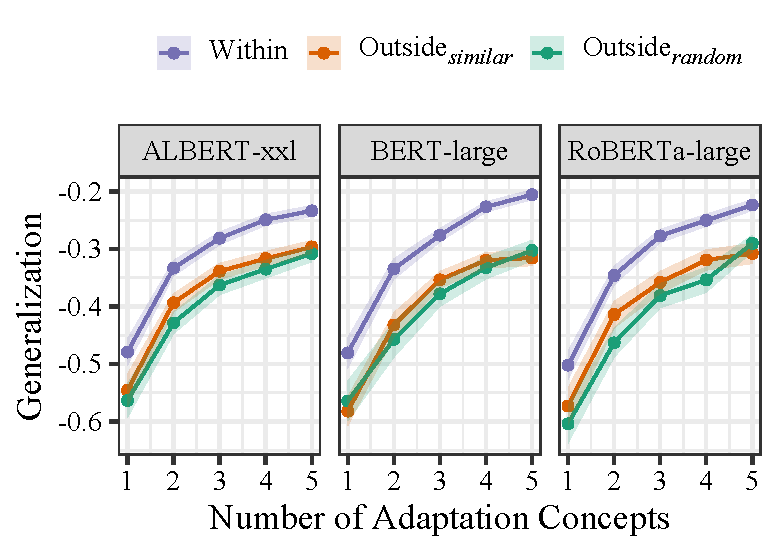
\includegraphics[width=\columnwidth]{generalization.pdf}
    \caption{Caption}
    \label{fig:gen}
\end{figure}

\begin{figure}
    \centering
    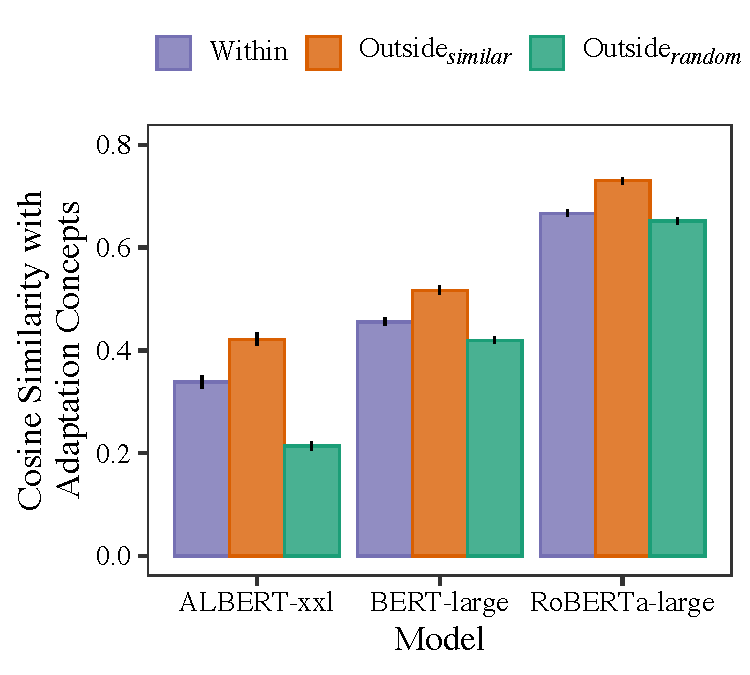
\includegraphics[width=\columnwidth]{cosine.pdf}
    \caption{Caption}
    \label{fig:cosine}
\end{figure}


\end{document}
